% ********* 中文 ********%%%
% 第4章 设计

% URN的首要目标是为提供一个统一的RDMA虚拟化框架,以适应混合虚拟环境。URN的第二个目标是高可管理性,服务器上的RDMA资源被集中管理和调度。URN的第三个目标高性能,虚拟RDMA的性能接近原生RDMA,因为网络性能是应用使用RDMA的核心诉求。第四个目标是尽可能保证兼容性,为对已有RDMA应用透明,对已有RDMA软件栈引入最小的代码改变量。

%为了实现上述目标,URN主要包含了vRNIC和URN core。vRNIC是对虚拟机和容器通用的虚拟RDMA网卡设备,URN core则是各主机服务器上的用于集中管理的虚拟层。在本章,我们介绍了URN中的一些关键性设计工作。

% 4.1  vRNIC设计

% vRNIC是一个虚拟RDMA设备,由前后端组成:前端在guest端, 负责为上层verb库提供接口并转发RDMA 命令;后端在主机端,以模拟guest对vRNIC的RDMA操作。

% 4.1.1 vRNIC后端

% 我们将vRNIC后端设计在主机用户空间,因为vRNIC后端在用户空间有诸多好处,具体细节可以见2.1节。

% 为了让vRNIC具备RDMA网卡的基本功能,vRNIC后端需要维护关于RDMA网卡的硬件属性,与物理RDMA网卡的出厂属性对应,例如RDMA地址,RDMA设备类型等。此外,在vRNIC的运行过程中,vRNIC后端中需要维护三方面的上下文:
% 1,来自guest的虚拟RDMA上下文信息;
% 2,由物理网卡创建的RDMA上下文,由vRNIC后端利用verbs库创建和维护;
% 3,虚拟RDMA上下文到物理RDMA上下文之间的对应关系。注意,对应关系是一对一的,用以guest应用中的各RDMA资源之间是隔离的,不会出现错误。

% 4.1.2 vRNIC前端

% 为了对虚拟机和容器通用,vRNIC前端为不同的虚拟场景提供统一的接口,用于连接guest中的应用和vRNIC后端。虚拟机和容器中有不同的vRNIC前端。 
% 在虚拟机中,vRNIC是外部设备,由虚拟机OS驱动。RDMA内核驱动包括与设备无关的OFED模块和设备相关的模块,OFED模块接受来自verbs库的命令,提供了内核层级的RDMA API;设备相关模块调用物理网卡设备的硬件接口,执行来自RDMA命令。为此,虚拟机中的vRNIC前端拦截RDMA内核驱动的RDMA命令,以同时支持RDMA内核层级的API和应用的Verbs API。具体做法是,虚拟机中需要一个自定义的设备相关的驱动模块,该模块用来配合RDMA内核驱动中原生的OFED模块,传递OFED的RDMA命令到vRNIC前端。
% 在容器中,vRNIC后端可以和容器应用共享主机操作系统,两者仅位于不同的命名空间。为了在用户空间完成vRNIC前端转发verbs命令的功能,容器的verbs库中与内核RDMA驱动交互的接口,被替换为vRNIC前端接口。Vers库中与内核交互的RDMA命令及参数,被劫持到vRNIC前端。然后通过vRNIC前端转发到vRNIC后端。

% 4.1  URN Core 设计

% 为了满足高可管理性的目标,每个主机服务器上都有一个集中的虚拟层URN core,其主要功能是实例化多个vRNIC实例,并管理各vRNIC之间的RDMA连接。

% 4.1.1 实例化vRNIC 

% 首先,在实例化vRNIC时,URN Core需要对vRNIC的不变属性进行初始化。vRNIC中的不变属性包括RDMA地址vGID,设备号等等。对于RDMA地址vGID,URN core会通过mgmt core进行协调和登记,以确保各vRNIC的RDMA地址等信息是不冲突的并维护在统一的数据库中。

% 其次,URN Core需要构建vRNIC后端与vRNIC前端(guest)之间的消息通道。对于容器来说,容器与vRNIC后端共享某一IPC命名空间,即可完成vRNIC前端与后端之间的消息交互。对于虚拟机来说,由于vRNIC后端在主机用户空间,而VM对应的hypervisor位于主机内核空间。为了避免guest的消息先拷贝到hypervisor层再到vRNIC后端,我们采用了vRNIC后端与guest共享内存的方式作为消息通道。具体来说,虚拟机内存区域对应的物理页面,与vRNIC后端之间是共享的。这样,guest中的任意RDMA消息,均可以直接由vRNIC后端获取,而无需进入到主机内核空间,同时也减少了消息从guest到vRNIC后端的延迟。

% 最后,URN core需要确保各vRNIC之间的消息通道是隔离的。在云环境中,同一主机上可能部署多个虚拟机或容器,该主机的URN core需要实例化多个vRNIC后端,以满足不同的guest实例。因此,需要确保各vRNIC之间的消息通道是隔离的,尤其是容器,由于其隔离性不如虚拟机彻底。如果多个容器和主机共享同一文件命名空间或IPC空间,那么,很容易通过扫描获取到其他容器或虚拟机vRNIC的消息通道。为此,URN core利用了文件命名空间的机制,将各vRNIC消息通道进行隔离。具体来说,无论虚拟机还是容器,vRNIC前后端之间的消息通道都是基于位于特定文件命名空间的共享文件的,对于别的guest实例,尤其是其他容器,是不可见的。

% 4.1.2 管理RDMA连接

%在云环境中,虚拟网络配置是实现很多功能的基础,例如多租户隔离、便携的虚拟机或容器迁移。虚拟网络配置包括了虚拟的网络地址,虚拟的路由规则以及其他软件定义的配置协议。URN在用户空间,支持灵活的虚拟RDMA网络配置。
% 首先,通过vRNIC后端控制接口,URN Core 可以用vRNIC后端维护的虚拟地址(例如vGID)配置vRNIC, 该地址可以通过vRNIC前端反映到客户端的应用程序中。

%其次,借助mgmt center 可以在每个URN Core中定义虚拟RDMA网络路由规则。每个vRNIC后端都配置了组ID, 路由规则定义为:{group ID1, group ID2, Policy}。一个关于查找路由规则的回调函数在实例化时注册到每个vRNIC后端。 这样,路由规则就可以实时地反映到服务器的所有vRNIC后端中。例如,如图4所示,容器1和容器2的vrnic被配置到同一组中,因此允许创建RDMA连接。作为对比,容器和虚拟机1是隔离的因为属于不同组。最后,vgid在物理RNIC中不能被识别,网络地址映射在vRNIC后端被创建和更新。如果路由规则允许,这对vgid将被转换成物理的gid来创建RDMA连接.

% 4.3 虚拟RDMA workflow

% 基于vRNIC和URN core,guest中可以实现透明的RDMA操作,其中包括控制路径和数据路径。在vRNIC中,控制路径和数据路径分离。其中,需要经过vRNIC后端,在vRNIC后端中创建RDMA源时会确保资源映射到guest应用。数据路径不需要经过vRNIC后端,直接在guest本地完成,避免了数据路径频繁的拷贝或切换开销。此外,vRNIC在原有的RDMA路径中加入了连接管理功能,以适应虚拟机和容器的云环境。

% 4.3.1 控制路径
% 控制路径依次包括虚拟设备打开,RDMA资源创建及映射(QP,CQ及MR等),虚拟RDMA连接建立等,主要包括了图4中的第1-7步。

%(1)虚拟设备打开
% 第一步:Guest应用获取并打开vRNIC设备。vRNIC后端会将vRNIC设备绑定到对应的物理网卡,然后打开真实的RDMA设备。

%(2) RDMA资源创建和映射
% RDMA资源按照位于的物理地址空间,分为内存资源(如QP)和设备资源(如门铃)。
% 对于内存资源(如QP,CQ和MR),在创建资源的过程中完成资源映射操作。无论是虚拟机还是容器,这类资源映射都是基于共享内存的方式来完成。具体如图4所示:

% 第二步:Guest应用创建QP/CQ等RDMA资源,此时,guest中的Verbs等库会指定QP或CQ的buffer。对于容器:在容器应用创建RDMA资源时,需要修改verbs库以使用共享内存作为QP或CQ的buffer,并将资源的共享路径传递给vRNIC后端。对于虚拟机:在虚拟机启动时,vRNIC后端已经与虚拟机所有内存完成了共享,因此,虚拟机中像原生verbs一样直接分配QP或CQ的buffer即可。vRNIC后端在收到guest的请求后,基于对应的共享内存使用物理RDMA网卡创建QP或CQ,然后返回对应的ID和元数据给guest。

% 第三步:Guest应用注册MR。由于MR的内存区域是由应用指定的,因此,为了维持透明性,在容器中,Verbs等库会重新映射MR区域到共享内存中。虚拟机中该步骤可以忽略,原因同第二步。同样的,vRNIC后端在收到该命令及参数后,会基于对应的共享内存注册MR,并返回地址和key等MR的信息。虚拟机和容器中的Verbs库,会记录guest中MR地址mem与vRNIC后端中MR地址s-mem,以及MR的key的三元组,用于后续的数据路径。

% 对于设备资源(如门铃),位于设备地址空间,由RDMA设备驱动管理。因此,无法在用户空间完成映射。为此,我们设计了一个用于映射RDMA设备资源且与host端RDMA内核驱动解耦的内核模块。vRNIC前端会将设备资源映射的命令和地址参数,转发到一个host内核模块,由该模块完成映射操作。具体细节见实现章节。 

%(3)虚拟RDMA连接建立

% 第四步:Guest应用查询vRNIC的vGID地址。vRNIC后端会获取绑定的物理RDMA网卡的GID,并记录(vGID,GID)对应关系。不过,vRNIC后端返回给guest的仍然是vGID。

% 第五步:Guest应用与远端交换vGID,QP ID及MR key等信息。 该步骤完全由应用程序完成,无需调用Verbs库。例如,应用中可以使用TCP socket来与远端guest应用完成这一系列信息的交换,
% 第六步:Guest应用基于远端vGID,QP ID及key与远端QP配对。该命令需要转发到vRNIC后端执行。vRNIC后端会先根据设置的路由表规则进行判断,如何远端vGID符合路由规则,就会将vGID转换成对应的GID,基于GID,QP ID及Key完成与远端vRNIC后端QP的配对。从vGID到GID的转换,实现了RDMA连接的网络虚拟化。
% 第七步:Guest应用将QP修改为连接状态,两端RDMA连接建立。在完成配对后,该命令会转发到vRNIC后端,由后端基于物理RDMA网卡的QP执行。由于QP在前面的第二步中已完成映射,在vRNIC后端QP处于连接状态后,guest中的QP同样会处于连接状态。

% 4.3.2 数据路径

% 数据路径发生在连接建立后,主要操作注册的MR中的内容。RDMA的数据路径包含双边操作(Send/Recv)和单边操作(Read,Write)等多种数据操作。数据路径主要包括了图中的第8和9步。

% (1) 双边操作
% 第八步:Guest应用发送MR中的数据。由于MR和QP已经完成了资源映射,此时,数据操作时的数据块(MR中)和工作请求(QPvs)可以直接由RDMA物理网卡访问。不过,工作请求中的地址信息仍然是guest中的地址,而第三步中创建MR时,物理网卡记录是vRNIC后端中的页表信息。因此,需要借助前面缓存的三元组信息,将工作请求中的guest地址转换为vRNIC后端地址,再填充到QP中。
% 第九步:Guest应用轮询CQ获取数据操作的完成事件。由于CQ已经完成了资源映射,此时,物理网卡中工作完成的通知会直接写入到guest的CQ中。

% (2) 单边操作
% 单边操作中,第八步和第九步仅在已建立RDMA连接的一端执行。单边操作的工作请求中包含了远端guest MR的内存地址及key,该信息在第五步已经由两端guest应用完成交换。由于远端应用注册MR时,其RDMA网卡中在缓存的是远端vRNIC后端的页表, 单边操作还需要知晓远端vRNIC后端的MR内存地址。为此,我们建立了一个分布式的KV数据库,存储各节点注册MR的映射关系。在guest执行单边操作时,将向分布式KV数据库查询,以获取远端vRNIC后端的MR内存地址,将其写入单边操作的工作请求中,从而实现单边操作。然而,由于频繁地查询分布式KV数据库会带来较高的延迟,为此,我们利用了RDMA数据收发的局部性,在guest本地建立了一个KV缓存区,以加速单边操作的性能。


% 4.3,虚拟RDMA管理
%  4.3.1 基本管理功能
%  在URN中,管理者可以通过mgmt center向不同的URN core下发各种策略,包括控制平面和数据平面。管理框架图如图5所示。
%  在控制路径:控制路径可以实现的管理功能包括路由管理、防火墙等。这些策略主要依靠RDMA资源,如QP进行控制。具体地,vRNIC后端按照mgmt下发的策略,可以在创建RDMA资源前执行策略,并在策略执行后将结果或资源信息返回给mgmt中维持各RDMA上下文信息的数据库中。
%  在数据路径:云环境中需要更多的管理功能,例如QoS,流量计费等策略。显然,这些策略依赖RDMA中数据路径的信息,例如消息大小。然而,在URN中,vRNIC前端和后端都在数据路径中被绕过。因此,我们应该将这些管理扩展到guest中的特定硬件库中,因为数据路径是在这个库中实现的。对于策略,可以通过管理中心进行配置和分发。注意,这些扩展需要所有客户机都信任库,并且这些修改应该包含在TCB(可信计算库)中。

%  4.3.2 讨论:
%    (1)虚拟机迁移:容器或虚拟机迁移在云中有很多好处,例如资源利用和故障转移。通过使用虚拟RDMA网络,URN可以支持脱机迁移,而无需为应用程序重新配置物理RDMA网络。具体来说,在重新启动迁移的虚拟实例后,应用程序可以通过相同的网络地址重建RDMA连接。唯一的工作是修改URN core中的地址映射.目前,由于RDMA应用程序中的内存区域在旁路或单侧通信下可能存在不确定性,因此对动态迁移仍然存在困难。该问题与URN无关.
%%%*********************%%%


\section{Design}
% URN的目标是为混合虚拟环境(指容器,虚拟机或虚拟机内容器等虚拟实例共存,甚至部署于同一服务器)提供一个统一的RDMA虚拟化框架。在这个框架里,服务器上的虚拟的或物理的RDMA资源仅被URN core 集中管理和调度。URN的第二个目标是虚拟RDMA的性能接近原生RDMA。第三个目标是对已有的RDMA应用程序透明,并且对RDMA软件栈引入最小的代码改变量。在本章,我们介绍了URN中的一些关键性设计工作。
The goal of URN is to provide a unified RDMA virtualization framework for hybrid virtual environments where containers, virtual machines and containers inside virtual machine could coexist, even on the same server. In this framework, virtual and physical RDMA resources on one server are solely managed and scheduled by the URN core. The second design goal of URN is that the performance of virtualized RDMA should be close to the native RDMA. The third design goal is to be transparent to the vanilla RDMA applications, and to bring minimal code changes to RDMA software stack. In this section, we introduce some key design details.

\subsection{URN Core}
% URN core被设计用来管理虚拟RDMA网络和物理RDMA资源在每个主机上, 包括实例化vRNIC后端,虚拟网络配置和RDMA资源限制等。同样的,URN实现在用户空间。
URN core is designed to manage the virtual and physical RDMA resources for the host, including instantiating vRNIC backends, virtual network configuration and RDMA resources limitation. Also, URN is in host user space for the same reasons in section xxx.

% URN core如何实例化vRNIC后端?
%注意到后端在主机用户空间,因此,URN core有必要建立一个消息通道在vRNIC和所有guest之间,因为URN core(主机用户空间) 是隔离虚拟机监视器或容器的。当guest需要vRNIC时,他们可以请求URN core在主机用户空间中实例化相应的后端。为了构建这个通道,我们使用了UNIX套接字对于虚拟机及容器环境。当虚拟机或容器需要一个新的vRNIC时,对套接字发出的实例化请求会被URN处理。为了快速支持多个实例化请求,这个过程中采用了反应器模式。
Recall that the vRNIC backends is in host user space, it is necessary to build a communication channel between URN and all guests, because the URN core is another process in host and the isolated with both containers and the hypervisor(VMs). When guests need a vRNIC, they can request the URN core to instantiate corresponding backend in host user space. To build this channel, we utilize the UNIX socket for both VMs and containers. When VMs or containers need a new vRNIC, the instantiating request to socket are deal with URN. To support multiple request rapidly, the reactor mode are adopted in the process. 


% URN core 对BE提供统一接口?
% 除了实例化vRNIC后端,URN core 还包括了管理功能:包括虚拟网络管理和硬件资源管理。 为了实现这些管理,URN core 首先要监控vRNIC后端的属性和上下文,并在URN核心中汇总信息(如资源内存映射)。为此,URN提供了记录RDMA上下文及属性的接口。在RNIC后端中,这些记录接口在Verbs命令执行后被调用,以更新记录信息;
%其次,URN core还提供了控制接口,并且用户定义的配置或控制策略可以部署到vRNIC后端。记录和控制接口都是回调函数,当vRNIC后端实例化时,它们被注册到vRNIC后端。接下来介绍虚拟网络配置和硬件资源管理:
Besides instantiating vRNIC backends, the URN core is also designed for the management: including virtual network and hardware resources. To achieve the management, at first, the attributes and contexts in vRNIC backends should be monitored and the information (e.g. resource memory mapping) should be summarized in URN core. Thus, the URN provides the recording interfaces about the attributes and contexts, and the interfaces are executed in vRNIC backends when the Verbs commands are executed; 
second, the control interfaces are also provided and user-defined configuration or control policies can be deployed into vRNIC backends. Both recording and control interfaces are lots of callback functions and they are registered into vRNIC backends when vRNIC backends instantiating. Later, the virtual network configurations an hardware resources management are introduced:

% 具体讲URN core提供了哪些管理功能:
% 1, 虚拟网络构建:在云环境中,虚拟网络配置是实现很多功能的基础,例如多租户隔离、便携的虚拟机或容器迁移。虚拟网络配置包括了虚拟的网络地址,虚拟的路由规则以及其他软件定义的配置协议。URN在用户空间,支持灵活的虚拟RDMA网络配置。
In clouds, virtual network configuration is important for lots of features, such as multi-tenant isolation and portable guest migrations. The virtual network configuration includes virtual network address, virtual network routing rules and other software-defined information. URN support flexible virtual RDMA network configurations in user space. 
%首先,通过vRNIC后端控制接口,URN可以用vRNIC后端维护的虚拟地址(例如vGID)配置vRNIC,该地址可以通过vRNIC前端反映到客户端的应用程序中。
First, through the control interface to vRNIC backends, URN can configure the vRNIC with virtual address (e.g. vGID) which maintained in vRNIC backends, and the address can be reflected into applications in the guest through the vRNIC frontend.
%其次,可以在每个URN核心中定义虚拟RDMA网络路由规则。每个vRNIC后端都配置了组ID,路由规则定义为:{group ID1, group ID2, Policy}。一个关于查找路由规则的回调函数在实例化时注册到每个vRNIC后端。这样,路由规则就可以实时地反映到服务器的所有vRNIC后端中。例如,如图~\ref{fig:route-config}所示,容器1和容器2的vrnic被配置到同一组中,因此允许创建RDMA连接。作为对比,容器和虚拟机1是隔离的因为属于不同组。最后,vgid在物理RNIC中不能被识别,网络地址映射在vRNIC后端被创建和更新。如果路由规则允许,这对vgid将被转换成物理的gid来创建RDMA连接.
Second, the virtual RDMA network routing rules can be defined in each URN core. Each vRNIC backend is configured with the group ID and the routing rules can be defined as: {Group ID1, Group ID2, Policy}. A callback function about lookuping routing rules is registered to each vRNIC backends when instantiating vRNIC backends. Thus, the routing rules can be reflected in real time for all vRNIC backends in the server. For example, as shown in Figure~\ref{fig:route-config}, the vRNICs for container 1 and container 2 are configured into the same group, thus RDMA connections are allowed to create. In contrast, the container 1 and VM 1 are isolated RDMA network because different groups. Finally, the vGIDs is not recognized in physical RNIC, and the network address mappings are created and updated in the vRNIC backends. If the routing rules allow, the pair of vGIDs will be translate to physical GIDs to create the RDMA connection.

\begin{figure}[!ht]
	\centering
	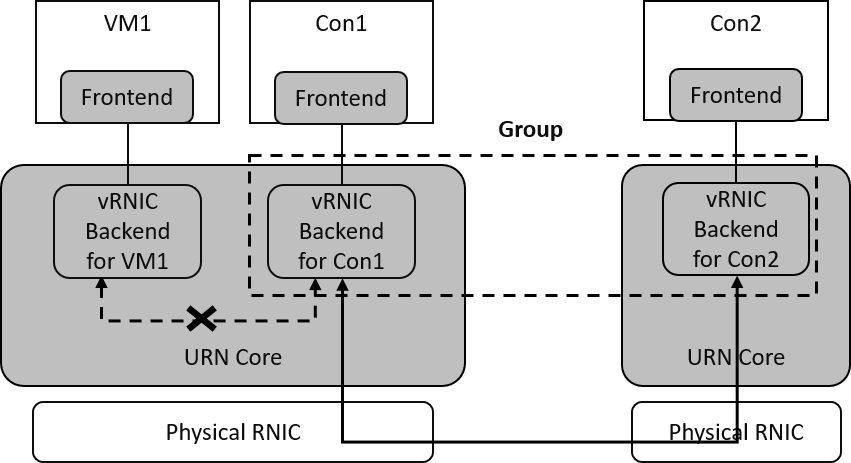
\includegraphics[width=1.0\linewidth]{images/route-config}
	\caption{Group Configuration and Routing: The vRNICs of container 1 and container 2 are configured in one group. Thus, two containers can create RDMA connections. And VM 1 are not allowed to create RDMA connections to containers in this figure because it is not added into the group. }
	\label{fig:route-config}
\end{figure}


\subsection{vRNIC Design}
% vRNIC是一个虚拟RDMA设备,包含前后端:前端在guest端, 负责为上层verb库提供接口并转发RDMA 命令;后端在主机端,通过与URN core或verbs库交互,以模拟guest对vRNIC的RDMA操作。 我们继承了控制和数据通道分离的哲学,和已有的RDMA虚拟化方案一样,如hyv和MasQ,控制路径上guest应用在本地的虚假RDMA上下文中执行verbs命令,并经过FE转发到BE维持的真实RDMA上下文中执行,之后将结果返回给guest;在数据路径上,将guest应用的RDMA资源与vRNIC BE上下文中的RDMA资源进行映射,guest应用的RDMA资源被注册到了物理网卡中,之后guest应用可以在本地直接使用RDMA资源进行数据操作。
vRNIC is a virtual RDMA device, which consists of the frontend and backend. The frontend forward the commands of Verbs library in the guest user space to backend. The backend execute the commands by interacting with the physical RNIC through Verbs library in host user space. We inherited the philosophy that the control path and data path of RDMA operations are virtualized in different ways\cite{pfefferle2015hybrid}\cite{he2020masq}\cite{kim2019freeflow}. On the control path, para-virtualization technique is used that control commands from the guest Verb library are served by the frontend and forwarded to backend. On the data path, direct-passthrough technique is used that applications in the guest environment can directly map and use physical RDMA resources so that no guest OS kernel or host virtualization layer is involved when sending and receiving network packages. The details of memory mapping implementations in URN framework is described in section 5 Implexxx.

\begin{figure}[!ht]
	\centering
	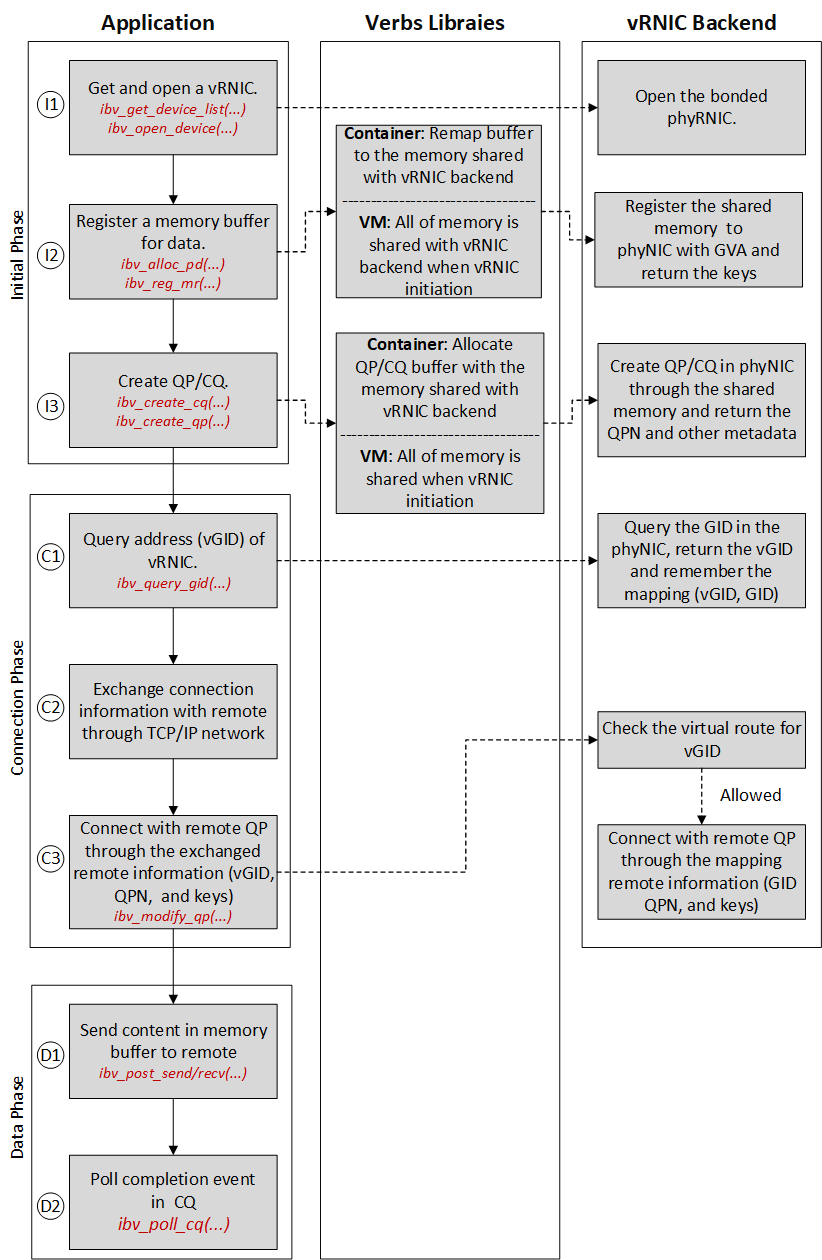
\includegraphics[width=1\linewidth]{images/RDMA-path.png}
	\caption{The Workflow of RDMA SEND operation}
	\label{fig:route-config}
\end{figure}


% 前端:
% vRNIC前端作为vRNIC的设备接口提供给guest中的verbs库。Verbs命令可以通过前端转发到后端。在虚拟机中,vRNIC前端位于guest内核空间,并模拟原生的RDMA内核驱动为上层的verbs库提供与原生一致的接口,例如设备总线,设备文件。因此,当虚拟机中的前端加载后,可以直接使用未修改的verbs库。这样的好处是让URN系统更加稳定。
%The vRNIC frontend acts as the device interface of the vRNIC for Verbs library in the guest environments. The Verbs commands can be forwarded from the frontend to the backend. 
The design of the vRNIC frontend is different in containers and VMs. In VMs, the frontend is located in the guest kernel space, and it exposes the interface of native RDMA kernel driver to Verbs library, in the form of device class and device file. Thus, unmodified Verbs library can be used in VMs and this makes URN framework transparent to the evolution of Verbs library in the virtual machine.
% 然而,在容器中,无法像虚拟机一样提供对verbs用户库透明的接口。这是因为,如果前端位于主机内核空间,并提供与原生RDMA内核驱动一致的虚拟设备接口给verbs用户库。这些虚拟设备接口将与原生的物理设备接口一同暴露给verbs用户库. verbs用户库在未经修改的前提下, 无法区分使用的接口是前端提供的还是RDMA内核驱动提供的。
However,in containers, it is impossible to provide the unmodified interface for Verbs library. Because, if the frontend in host kernel space provides the same interfaces same as RDMA kernel driver. Note that both the virtual device interfaces and physical device interfaces are exposed to Verbs library in containers, and Verbs cannot distinguish them without extra modification in containers.  
% 因此,我们直接将前端实现在用户空间,作为一个用户库提供,并链接到Vers库。特别的,Verbs库中与设备接口相关的系统调用被替换为与前端交互的函数调用。容器应用程序在链接这个前端库后便可以转发verbs命令到后端。
%因此,容器前端的另一个好处是与Verbs交互完全在用户空间,没有系统调用开销。最后,注意虚拟机和容器的前端都是设备无关的,因为它们仅仅与通用的Verbs库及后端交互。
Thus, the frontend for containers is in user space, provided as a costumed library, and linked to Verbs library. In specific, in Verbs library, the origin device interface are replaced with the function call to the frontend. The Verbs commands can be forwarded to vRNIC backends after loading the frontend library. 
Thus, another advantage is that the interact with upper Verbs library is wholly finished in user space without the overhead of system calls. Finally, note that all frontends is hardware-independent because they only interact with the hardware-independent Verbs library and backends.


% 后端:后端在哪,为什么用户空间?
% 在URN中,vRNIC 后端实现在主机的用户空间作为一个虚拟设备。在用户空间主要有三方面的优势:1y用户空间更适合管理:开发管理功能,在用户空间更加简单并且灵活;2,用户空间的稳定性更好:由于用户空间不存在面向内核的攻击面;3,用户空间的兼容性更好,因为用户空间对于不同的系统架构、内核版本和设备内核驱动兼容.
 In URN, the vRNIC backend locates in the host user space as a virtual device. There are three advantages for vRNIC backend in user space: first, user space is more suitable for management: the develop of management functions is easier and more flexible in user space; second, user space provides higher stability: the attack surface for kernel is not in user-space; third, the user space provides higher compatibility because it is often independent on specific APIs (e.g. system architecture, kernel version and device kernel driver).

% 后端中需要维持哪些内容,为什么要维护?
% 后端作为虚拟设备,为guest提供的RDMA服务最终仍然需要由通过使用物理RNIC来完成。因此,在后端中,需要维护三方面的信息:1, 来自guest的虚拟的RDMA上下文信息: 该信息在接受前端请求时便可以记录下来,例如guest中应用的MR的虚拟地址GVA;2,主机中的真实RDMA上下文信息:这些信息直接通过verbs库来维持,并且能被物理网卡设备识别;3,两者的映射关系。在解析前端命令并调用Verbs库后,进行指定。基于上述信息,后端可以通过与UNR core进行交互,来实现对虚拟RDMA网络的管理以及对vRNIC使用硬件资源的统一管控。关于管理功能主要在URN core章节介绍。
As a virtual device, the RDMA service provided by the backend should be executed through the physical RNIC. Thus, there are three aspects of information need to be maintained: 
a) attributes for the virtual RDMA contexts in the guest environment: they can be recorded when the commands are received from the frontend in the guest, e.g. the GVA (guest virtual address) of MR in the application inside the guest.
b) attributes for the physical RDMA contexts in the host: they is maintained through the Verbs library and can be recognized by physical RNIC, e.g. the HVA (Host Virtual Memory) of MR in the host.
c) the mappings between virtual and physical attributes: the mapping relationship are assigned when the Verbs commands from the frontend are executed. 
Based on the above information, the vRNIC backend can interact with the URN core to achieve the virtual RDMA network management and the hardware source management. And the management are mainly introduced in section xxx.

\begin{figure}[!ht]
	\centering
	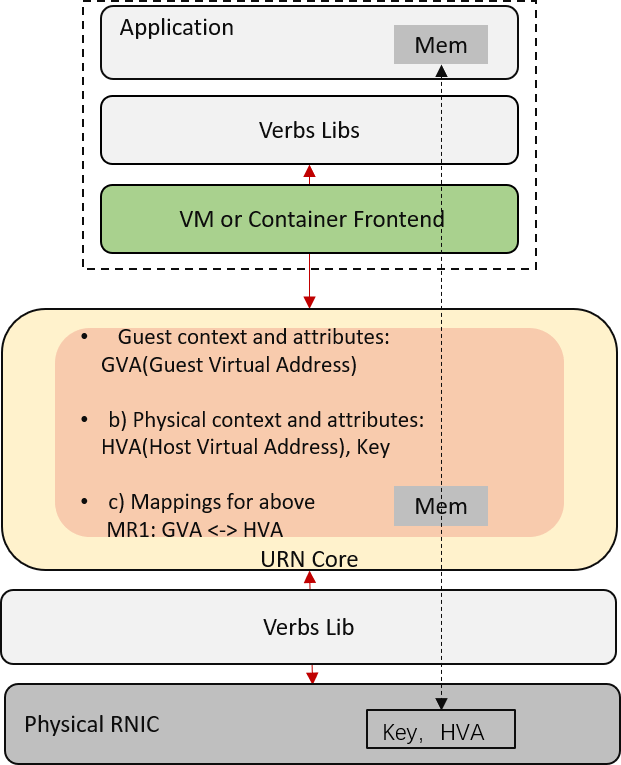
\includegraphics[width=0.8\linewidth]{images/vrnic-backend.png}
	\caption{The information maintained in vRNIC backends}
	\label{fig:route-config}
\end{figure}


\subsection{Management}

\begin{figure}[!ht]
	\centering
	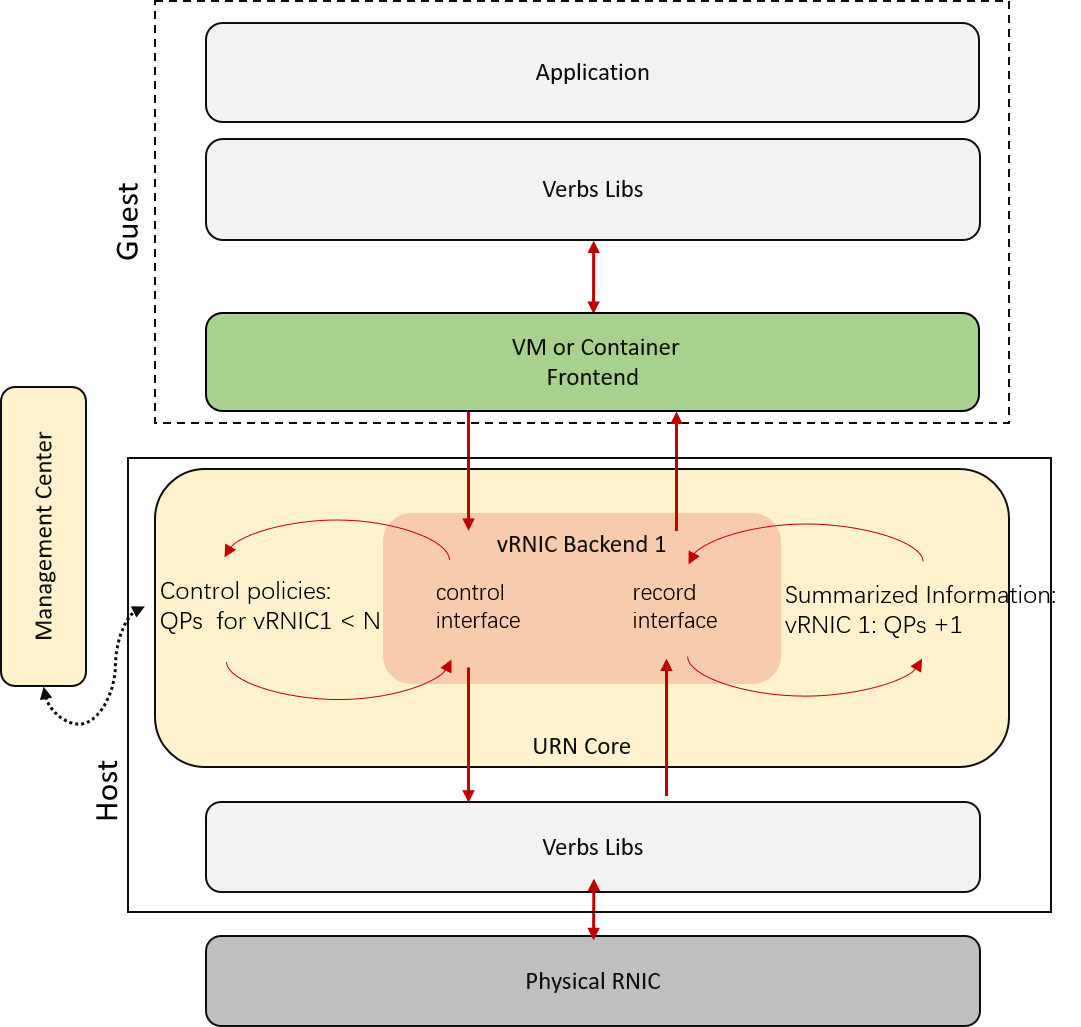
\includegraphics[width=1\linewidth]{images/urn-interface.png}
	\caption{Management Architecture in URN}
	\label{fig:framework-overview}
\end{figure}

% 2 对硬件资源的管理: 主要分为两部分,一对vRNIC使用的资源进行限制,以QP资源为例子;二,对硬件资源通过灵活映射的方式提高利用率, 以VF映射为例子。
% 硬件资源管理是URN core的另一个重要特性。在URN内核中,每个vRNIC使用的硬件资源都是受限的。例如,QP是RDMA的关键资源,创建过多的QP可能会降低RDMA的性能。URN核心还可以通过记录接口监视服务器中的所有QPs。另外,可以在URN core中定义QPs的最大值,也可以将熔断策略注册到vRNIC后端。当QPs对于vRNIC过多时,后续的creat_qp将被中止。
Hardware resource management is another important feature in URN core. In URN core, hardware resources can be limited for each vRNIC. For example, QP is the key resource in RDMA and many QPs may decrease the performance of RDMA. The URN core can monitoring all QPs in the server through the recording interface. The maximum of QPs can be defined in URN core and the fusing policy can be also registered to vRNIC backends. When QPs are excessive for a vRNIC, the subsequent creat\_qp will be aborted. 
% 此外,URN核心中可以灵活地利用硬件资源。在URN core中,所有硬件资源的状态信息都可以通过各个vRNIC后端或Verbs库进行汇总。通过灵活地将虚拟RDMA上下文映射到物理硬件资源上,可以实现硬件资源的高效利用。例如,VFs可用于云中的性能隔离。但是VFs是有限的,有最大值,如63~126,而且VFs的分配是静态的。因此,如果客户机数量大于服务器中的VFs,则无法满足每个客户机的性能隔离。为了解决这个问题,URN core可以灵活地将VFs映射到vRNIC,实现每个客户端的性能隔离。当URN core发现vRNIC处于空闲状态时,URN core便会释放该vRNIC的VF, 并将其分配给其他已经就绪的vRNIC。
Besides, hardware resources can be utilized flexible in URN core. In URN core, the status of all hardware resources can be summarized by the vRNIC backends and the Verbs library. By flexibly mapping virtual RDMA contexts to physical hardware resources, efficient utilization of hardware resources can be achieved. For example, the VFs can be used for performance isolation in clouds. But VFs is limited with maximum e.g. 63~126, and the allocation of VFs is static. Thus, if the guests is more than the VFs in a server, the performance isolation for each guest is not meet. To solve this problem, the URN core can flexibly map VFs to vRNICs to achieve the performance isolation for each guest. If the URN core finds that the vRNIC is idle, the VF of the vRNIC is released by URN core and it can be allocated to another ready vRNIC.



% 4.4 discussion 

% (2)虚拟实例迁移:容器或虚拟机迁移在云中有很多好处,例如资源利用和故障转移。通过使用虚拟RDMA网络,URN可以支持脱机迁移,而无需为应用程序重新配置物理RDMA网络。具体来说,在重新启动迁移的虚拟实例后,应用程序可以通过相同的网络地址重建RDMA连接。唯一的工作是修改URN core中的地址映射.目前,由于RDMA应用程序中的内存区域在旁路或单侧通信下可能存在不确定性,因此对动态迁移仍然存在困难。该问题与URN无关.
 Virtual Instances Migration: Migration of containers or VMs has many benefits in clouds, e.g. resource utilization and fail-over. With the virtual RDMA network, URN can support offline migration without reconfiguring the physical RDMA network for applications. In specific, after rebooting the migrated virtual instance, the application can rebuild the RDMA connection through the same network address. The only work is modifying the address mapping in URN core. Currently, for live migrations, it is still hard because memory regions in RDMA application may be uncertain under bypassing or one-side communication. And the problem is unrelated to URN.
